% Fig 5 (fig:perf_distribution): standalone source for the paper figure.
% Data: the boxplot five-number summaries below are hardcoded (from the depth-4, Pop-150,
% n=30 per-generation-cost distributions; no separate extract script).
% Build: pdflatex perf_distribution.tex  ->  perf_distribution.pdf  (see build_figures.sh)
% width=347.12pt matches the LLNCS \textwidth of the paper.
\documentclass[border=2pt]{standalone}
\usepackage[T1]{fontenc}
\usepackage{amsmath,amssymb}
\usepackage{tikz}
\usetikzlibrary{shapes.geometric, arrows.meta, positioning, patterns, calc}
\usepackage{pgfplots}
\pgfplotsset{compat=1.18}
\usepgfplotslibrary{fillbetween}
\usepgfplotslibrary{statistics}
% Okabe-Ito colorblind-safe palette (Wong 2011, Nature Methods)
\definecolor{oiblue}{HTML}{0072B2}
\definecolor{oiorange}{HTML}{E69F00}
\definecolor{oiskyblue}{HTML}{56B4E9}
\definecolor{oigray}{HTML}{999999}
\definecolor{oivermillion}{HTML}{D55E00}
\definecolor{oigreen}{HTML}{009E73}
\definecolor{oipurple}{HTML}{CC79A7}
\begin{document}
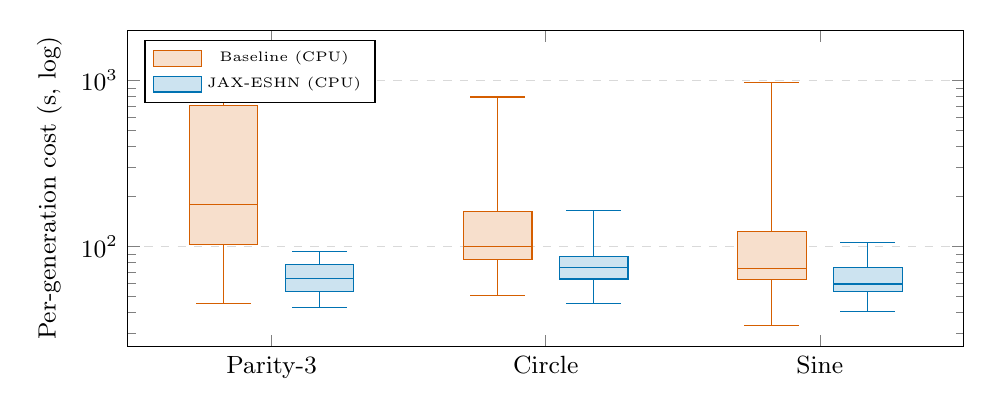
\begin{tikzpicture}
\begin{axis}[
    boxplot/draw direction=y,
    boxplot/box extend=0.5,
    ymode=log,
    width=347.12pt,
    height=5.6cm,
    ylabel={Per-generation cost (s, log)},
    ymin=25, ymax=2000,
    xmin=0.3, xmax=6.4,
    xtick={1.35, 3.35, 5.35},
    xticklabels={Parity-3, Circle, Sine},
    tick label style={font=\small},
    label style={font=\small},
    ymajorgrids=true,
    grid style={dashed, gray!30},
    legend style={at={(0.02,0.97)}, anchor=north west, font=\tiny},
]
% Baseline (CPU): oivermillion
\addplot+[boxplot prepared={draw position=1, lower whisker=45.2, lower quartile=102.4, median=179.1, upper quartile=707.6, upper whisker=1155}, oivermillion, solid, fill=oivermillion!20, area legend] coordinates {};
\addlegendentry{Baseline (CPU)}
\addplot+[boxplot prepared={draw position=3, lower whisker=51.0, lower quartile=83.5, median=99.4, upper quartile=161.4, upper whisker=792.6}, oivermillion, solid, fill=oivermillion!20, forget plot] coordinates {};
\addplot+[boxplot prepared={draw position=5, lower whisker=33.4, lower quartile=63.4, median=73.9, upper quartile=123.3, upper whisker=968.3}, oivermillion, solid, fill=oivermillion!20, forget plot] coordinates {};
% JAX-ESHN (CPU backend): oiblue
\addplot+[boxplot prepared={draw position=1.7, lower whisker=43.0, lower quartile=53.6, median=64.5, upper quartile=78.2, upper whisker=93.8}, oiblue, solid, fill=oiblue!20, area legend] coordinates {};
\addlegendentry{JAX-ESHN (CPU)}
\addplot+[boxplot prepared={draw position=3.7, lower whisker=45.4, lower quartile=63.8, median=74.8, upper quartile=87.1, upper whisker=163.8}, oiblue, solid, fill=oiblue!20, forget plot] coordinates {};
\addplot+[boxplot prepared={draw position=5.7, lower whisker=40.8, lower quartile=53.6, median=59.5, upper quartile=74.8, upper whisker=105.9}, oiblue, solid, fill=oiblue!20, forget plot] coordinates {};
\end{axis}
\end{tikzpicture}
\end{document}
